\section{\textbf{Experimental Results}}
Our proposed suspicious text detection system is tested with logistic regression, naive bayes, SVM,  KNN and decision tree classification algorithms. Table \ref{AE} represents accuracy and error rate of these algorithms on our dataset.\par
\renewcommand{\arraystretch}{1.5}
\begin{table}[h!]
\begin{center}
\caption{Evaluation Summary}
\begin{tabular}{||m{4.65cm} | m{1.4cm}| m{1.35cm}||}
\hline
     Classification Algorithm & Accuracy  & Error  \\
\hline
\hline
    Naive Bayes \cite{yoo2015classification} & 0.85 & 0.15\\
\hline 
    SVM (Linear Kernel) \cite{wei2012text} & 0.91 & 0.09\\
\hline 
    SVM (RBF Kernel) \cite{villmann2017can}& 0.90 & 0.10\\
\hline 
    Logistic Regression\cite{sharma2015active} $_{proposed}$ & 0.92 & 0.08\\
\hline
    K-Nearest Neighbor \cite{harisinghaney2014text}& 0.73 & 0.27\\
\hline
    Decision Tree \cite{chavan2014survey}& 0.88 & 0.12\\
\hline
\end{tabular}
\label{AE}
\end{center}
\end{table}
Table \textbf{\ref{prr}} shows average precision, recall and $F_1$ score of different classification algorithms used in our model.
\renewcommand{\arraystretch}{1.5}
\begin{table}[h!]
\begin{center}
\caption{Performance Comparison}
\begin{tabular}{||m{3.3cm} | m{1.25cm}| m{1.2cm}| m{1.3cm}||}
\hline
     Classification Algorithm & Precision & Recall & $F_1$ score \\
\hline
\hline
    Naive Bayes & 0.89 & 0.85 & 0.85\\
\hline 
    SVM (Linear Kernel) & 0.91 & 0.91 & 0.91\\
\hline 
    SVM (RBF Kernel) & 0.90 & 0.91 & 0.90\\
\hline 
    Logistic Regression$_{(proposed)}$ & 0.91 & 0.93 & 0.93\\
\hline
    K-Nearest Neighbor & 0.82 & 0.73 & 0.70\\
\hline
    Decision Tree & 0.88 & 0.92 & 0.89\\
\hline
\end{tabular}
\label{prr}
\end{center}
\end{table}

For all of the algorithms we used similar number of training and test documents. From table \textbf{\ref{AE}} and \textbf{\ref{prr}}, we can see that logistic regression and support vector machine algorithms are performing up to the mark on our dataset. Naive bayes and decision tree also doing really well. But accuracy of k-nearest neighbour is really poor compared to other algorithms.\par
\vspace{0.2cm}

Now, we will analyze classification report of logistic regression. Classification report gives us precision, recall and $F_1$ score of each class which is really helpful to examine and find out shortcomings of the algorithm.
Table \textbf{\ref{lr}}  shows classification report of logistic regression for our system. 

%%% Comment out several tables %%%%%%
\iffalse
\renewcommand{\arraystretch}{1.1}
\begin{table}[h!]
\begin{center}
\caption{Classification Report (Naive Bayes)}
\begin{tabular}{|m{2.8cm} | m{1.5cm}| m{1.3cm}| m{1.5cm}|}
\hline
     & Precision & Recall & $F_1$ score\\
\hline
     Suspicious & 1.00 & 0.71 & 0.83\\
\hline 
     Non suspicious  & 0.76 & 1.00 & 0.87\\
\hline 
     avg./total & 0.89 & 0.85 & 0.85\\
\hline
\end{tabular}
\label{NBC}
\end{center}
\end{table}

\begin{table}[h!]
\begin{center}
\caption{Classification Report (SVM Linear Kernel)}
\begin{tabular}{|m{2.8cm} | m{1.5cm}| m{1.3cm}| m{1.5cm}|}
\hline
     & Precision & Recall & $F_1$ score\\
\hline
     Suspicious & 0.91 & 1.00 & 0.91\\
\hline 
     Non suspicious  & 1.00 & 0.90 & 0.91\\
\hline 
     avg./total & 0.91 & 0.91 & 0.91\\
\hline
\end{tabular}
\label{SVML}
\end{center}
\end{table}

\begin{table}[h!]
\begin{center}
\caption{Classification Report (SVM RBF Kernel)}
\begin{tabular}{|m{2.8cm} | m{1.5cm}| m{1.3cm}| m{1.5cm}|}
\hline
     & Precision & Recall & $F_1$ score\\
\hline
     Suspicious & 0.90 & 0.99 & 0.90\\
\hline 
     Non suspicious  & 0.99 & 0.89 & 0.91\\
\hline 
     avg./total & 0.90 & 0.91 & 0.90\\
\hline
\end{tabular}
\label{SVMR}
\end{center}
\end{table}
\fi
%%% Showing logistic regression table %%%%%%%%%%%%%% 
\renewcommand{\arraystretch}{1.6}
\begin{table}[h!]
\begin{center}
\caption{Classification Report (Logistic Regression)}
\begin{tabular}{||m{3.1cm} | m{1.4cm}| m{1.2cm}| m{1.4cm}||}
\hline
     Class $(C)$& Precision & Recall & $F_1$ score\\
\hline
\hline
     Suspicious $(C_s)$ & 0.92 & 1.00 & 0.93\\
\hline 
     Non suspicious $(C_{ns})$  & 1.00 & 0.93 & 0.93\\
\hline 
     avg./total & 0.91 & 0.93 & 0.93\\
\hline
\end{tabular}
\label{lr}
\end{center}
\end{table}

%%% Comment out another table of block %%%%%
\iffalse
\begin{table}[h!]
\begin{center}
\caption{Classification Report (K-Nearest Neighbor)}
\begin{tabular}{|m{2.8cm} | m{1.5cm}| m{1.3cm}| m{1.5cm}|}
\hline
     & Precision & Recall & $F_1$ score\\
\hline
     Suspicious & 0.65 & 1.00 & 0.79\\
\hline 
     Non suspicious  & 1.00 & 0.44 & 0.61\\
\hline 
     avg./total & 0.82 & 0.73 & 0.70\\
\hline
\end{tabular}
\label{tknn}
\end{center}
\end{table}

\begin{table}[h!]
\begin{center}
\caption{Classification Report (Decision Tree)}
\begin{tabular}{|m{2.8cm} | m{1.5cm}| m{1.3cm}| m{1.5cm}|}
\hline
     & Precision & Recall & $F_1$ score\\
\hline
     Suspicious & 0.91 & 0.89 & 0.90\\
\hline 
     Non suspicious  & 0.88 & 0.90 & 0.89\\
\hline 
     avg./total & 0.90 & 0.90 & 0.90\\
\hline
\end{tabular}
\label{tdct}
\end{center}
\end{table}
\fi
From the above table, we get the value of precision for suspicious class $(C_s)$ is $0.92$. It means the number of texts logistic regression classified as suspicious among them $92\%$ are actually suspicious. It can correctly classify all non suspicious text $(C_{ns})$. From the recall value we get true positive rate for $(C_s)$ is $1.00$ and for $(C_{ns})$ is $0.93$ respectively. Logistic regression gives similar $F_1$ score for both class that is $0.93$. Average precision, recall and $F_1$ score is calculated by using mean of $C_s$ and $C_{ns}$.\par

We use precision-recall curves and receiver operating characteristics (ROC) curves to evaluate our model. Precision-recall curve summarizes the trade-off between the true positive rate and the positive predictive value  while ROC curve summarizes trade-off between the true positive rate and false positive rate for a predictive model using different probability thresholds. \textbf{Fig.} \ref{flr} to \textbf{Fig.} \ref{fdct} shows precision-recall and ROC curves for the algorithms used to test our system.

\begin{figure}[H]
\centering
\subcaptionbox{precision-recall}{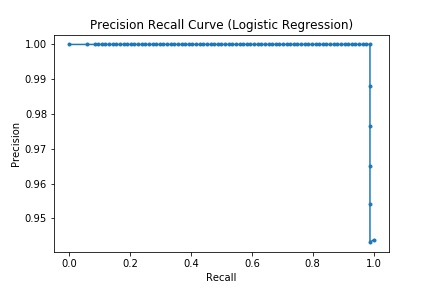
\includegraphics[scale=0.29]{Figures/PRLR.jpg}}%
\hfill % <-- Seperation
\subcaptionbox{ROC}{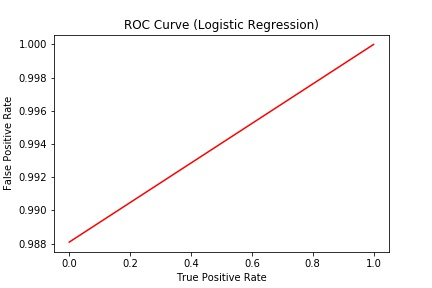
\includegraphics[scale =0.29]{Figures/ROCLR.jpg}}%
\caption{Result of Logistic Regression}
\label{flr}
\end{figure}
\noindent
\text{Fig.} \ref{flr} shows that we get high precision and recall for different threshold values with logistic regression. There exists a linear relationship between true positive rate and  false positive rate.
\begin{figure}[H]
\centering
\subcaptionbox{precision-recall}{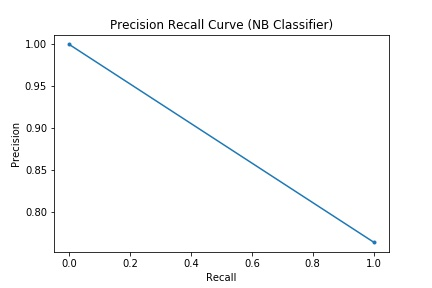
\includegraphics[scale=0.29]{Figures/PRN.jpg}}%
\hfill % <-- Seperation
\subcaptionbox{ROC}{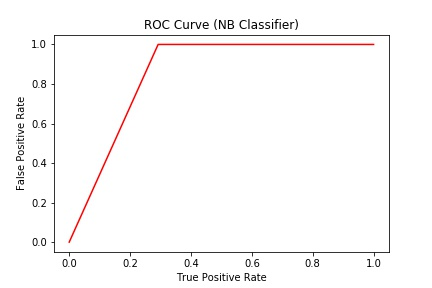
\includegraphics[scale =0.29]{Figures/ROCN.jpg}}%
\caption{Result of Naive Bayes Classifier}
\label{prrn}
\end{figure}
\noindent
For naive bayes classifier increase in recall causes linear decrease in precision. Here false positive rate become constant as true positive rate exceeds a certain threshold value.   
\begin{figure}[H]
\centering
\subcaptionbox{precision-recall}{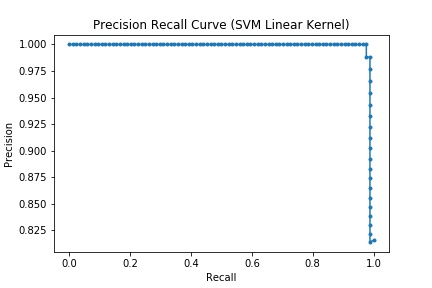
\includegraphics[scale=0.29]{Figures/PRSL.jpg}}%
\hfill % <-- Seperation
\subcaptionbox{ROC}{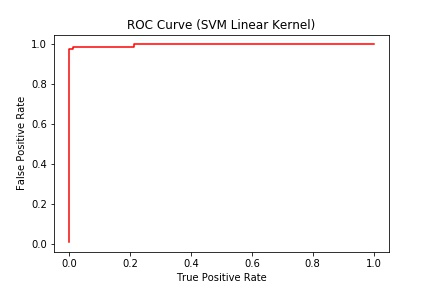
\includegraphics[scale =0.29]{Figures/ROCSL.jpg}}%
\caption{Result of SVM (Linear Kernel)}
\label{slk}
\end{figure}

\begin{figure}[H]
\centering
\subcaptionbox{precision-recall}{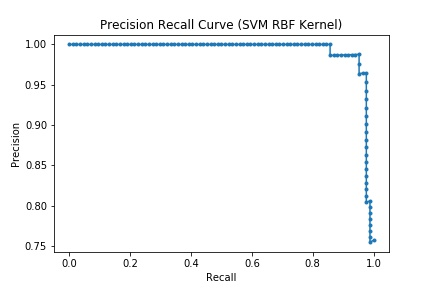
\includegraphics[scale=0.29]{Figures/PRSR.jpg}}%
\hfill % <-- Seperation
\subcaptionbox{ROC}{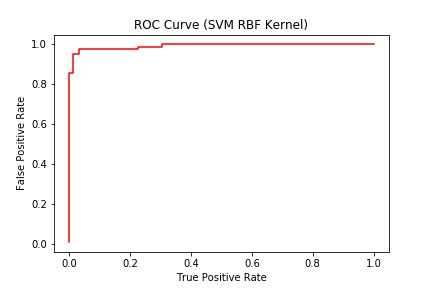
\includegraphics[scale =0.29]{Figures/ROCSR.jpg}}%
\caption{Result of SVM (RBF Kernel)}
\label{svr}
\end{figure}
\noindent
\textbf{Fig.} \ref{slk} and \textbf{Fig.} \ref{svr} shows the result of SVM using different kernel trick. Both algorithm give high precision, recall, true positive rate and false positive rate for different threshold values.  

\begin{figure}[H]
\centering
\subcaptionbox{precision-recall}{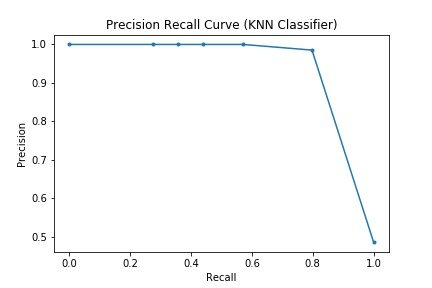
\includegraphics[scale=0.29]{Figures/PRKNN.jpg}}%
\hfill % <-- Seperation
\subcaptionbox{ROC}{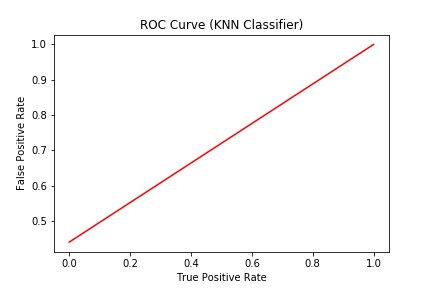
\includegraphics[scale =0.29]{Figures/ROCKNN.jpg}}%
\caption{Result of K-Nearest Neighbor}
\label{fknn}
\end{figure}

\begin{figure}[H]
\centering
\subcaptionbox{precision-recall}{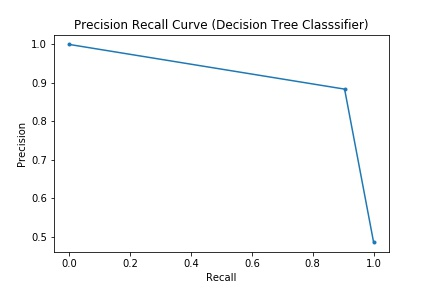
\includegraphics[scale=0.29]{Figures/PRDCT.jpg}}%
\hfill % <-- Seperation
\subcaptionbox{ROC}{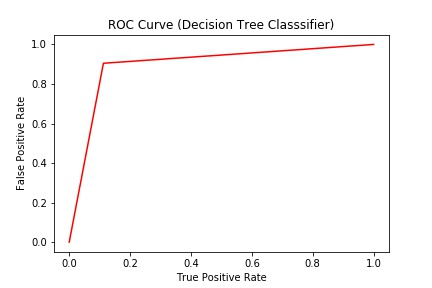
\includegraphics[scale =0.29]{Figures/ROCDCT.jpg}}%
\caption{Result of Decision Tree}
\label{fdct}
\end{figure}

\noindent
For both k-nearest neighbor and decision tree after a certain value of recall these is a rapid decrease in precision.   
\textbf{Fig.} \ref{fig:out} shows sample input and corresponding output in our system.
\begin{figure}[h!]
\centering
  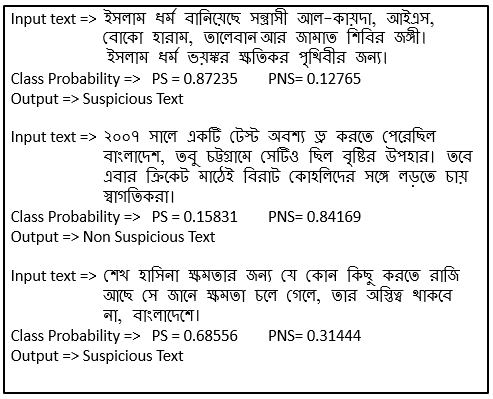
\includegraphics[height=6.8cm, width=8.8cm]{Figures/sout.PNG}
  \caption{ Output in System Environment}
  \label{fig:out}
\end{figure}

For a sample input text our model gives class probability for both suspicious class $(C_s)$ and non suspicious class $(C_{ns})$. A text is marked with that class $(C)$ which has higher probability. In the first example suspicious class probability is $P_s = 0.87235$ and non suspicious class probability is $P_{ns} = 0.12765$ so this text is a suspicious text.
